\documentclass[10pt, twoside, a4paper,openany]{book}
\usepackage{macra_xelatex}


\begin{document}
% strony generowane z moja.pg
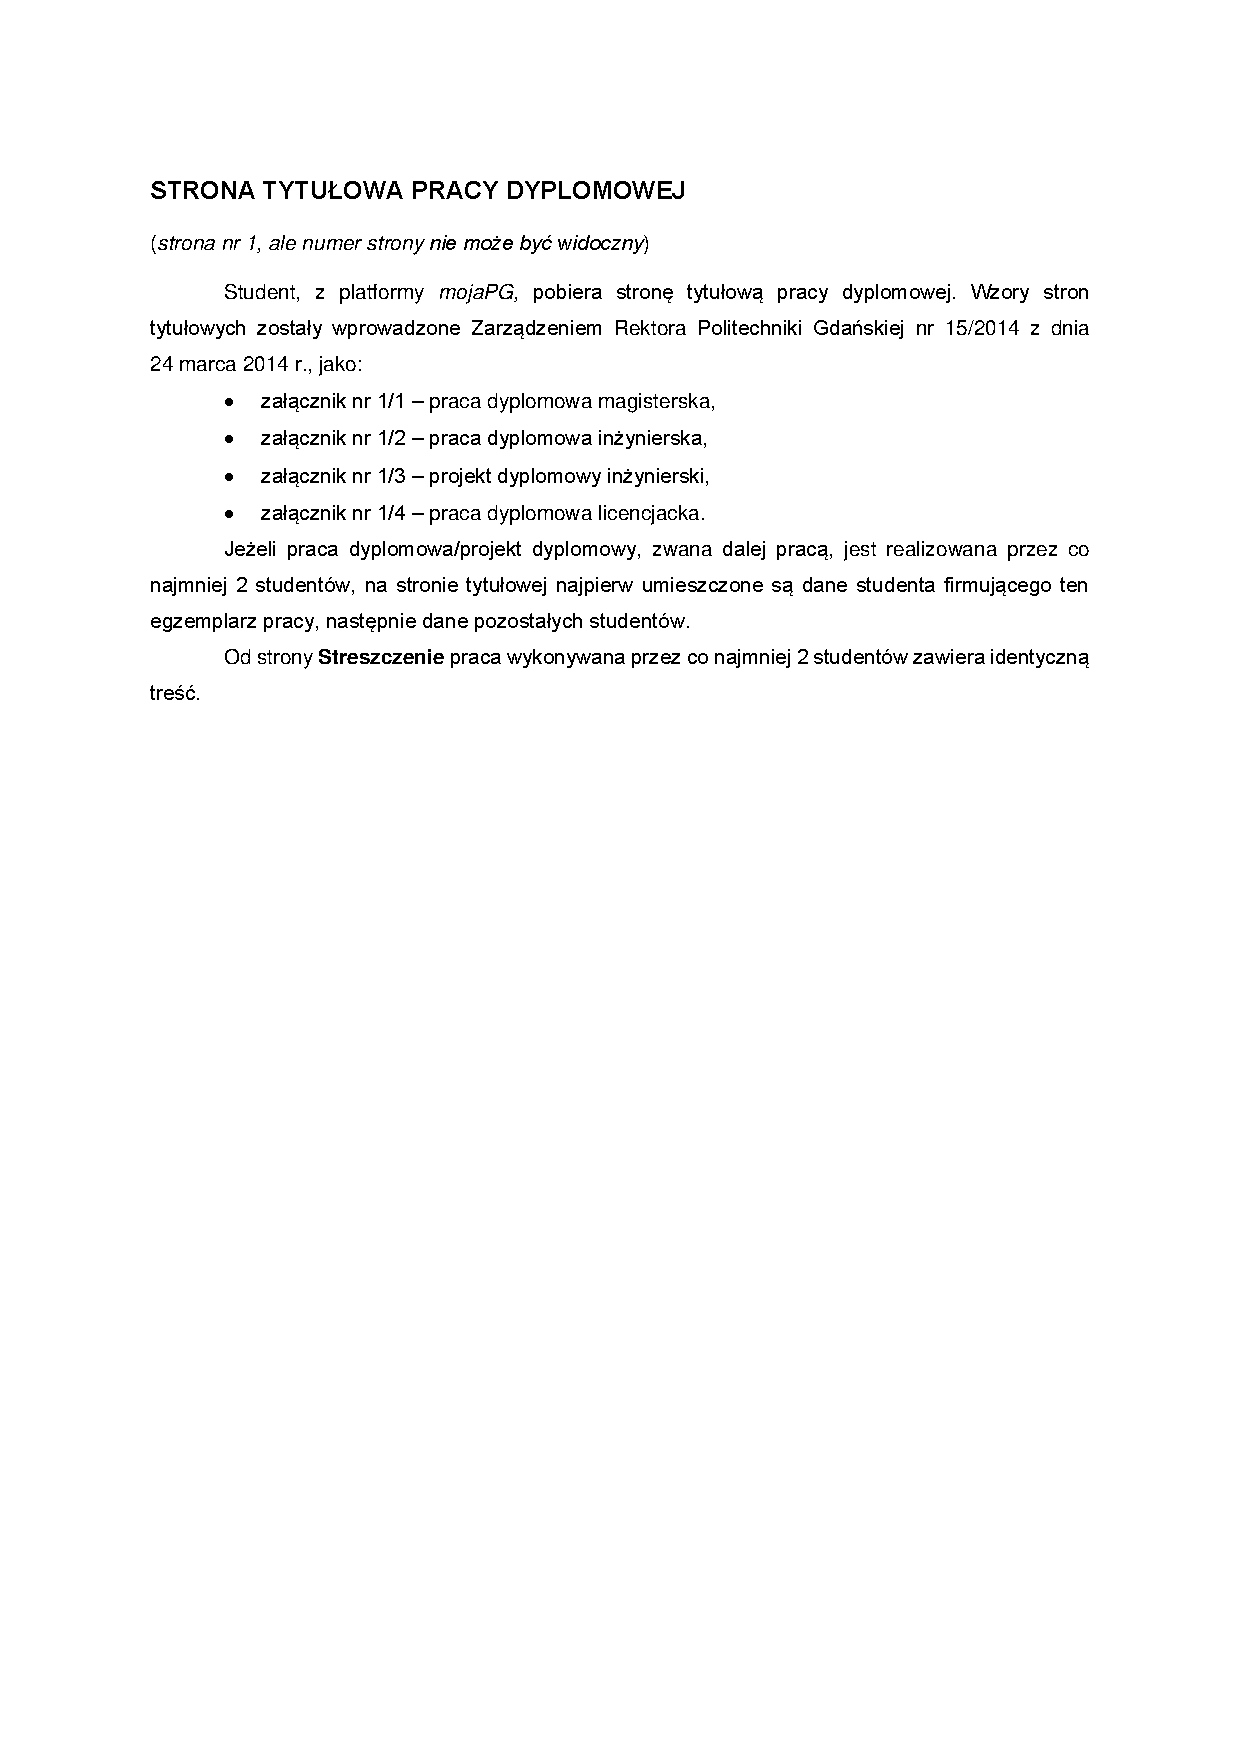
\includepdf{Chapters/Strona_tytulowa.pdf}
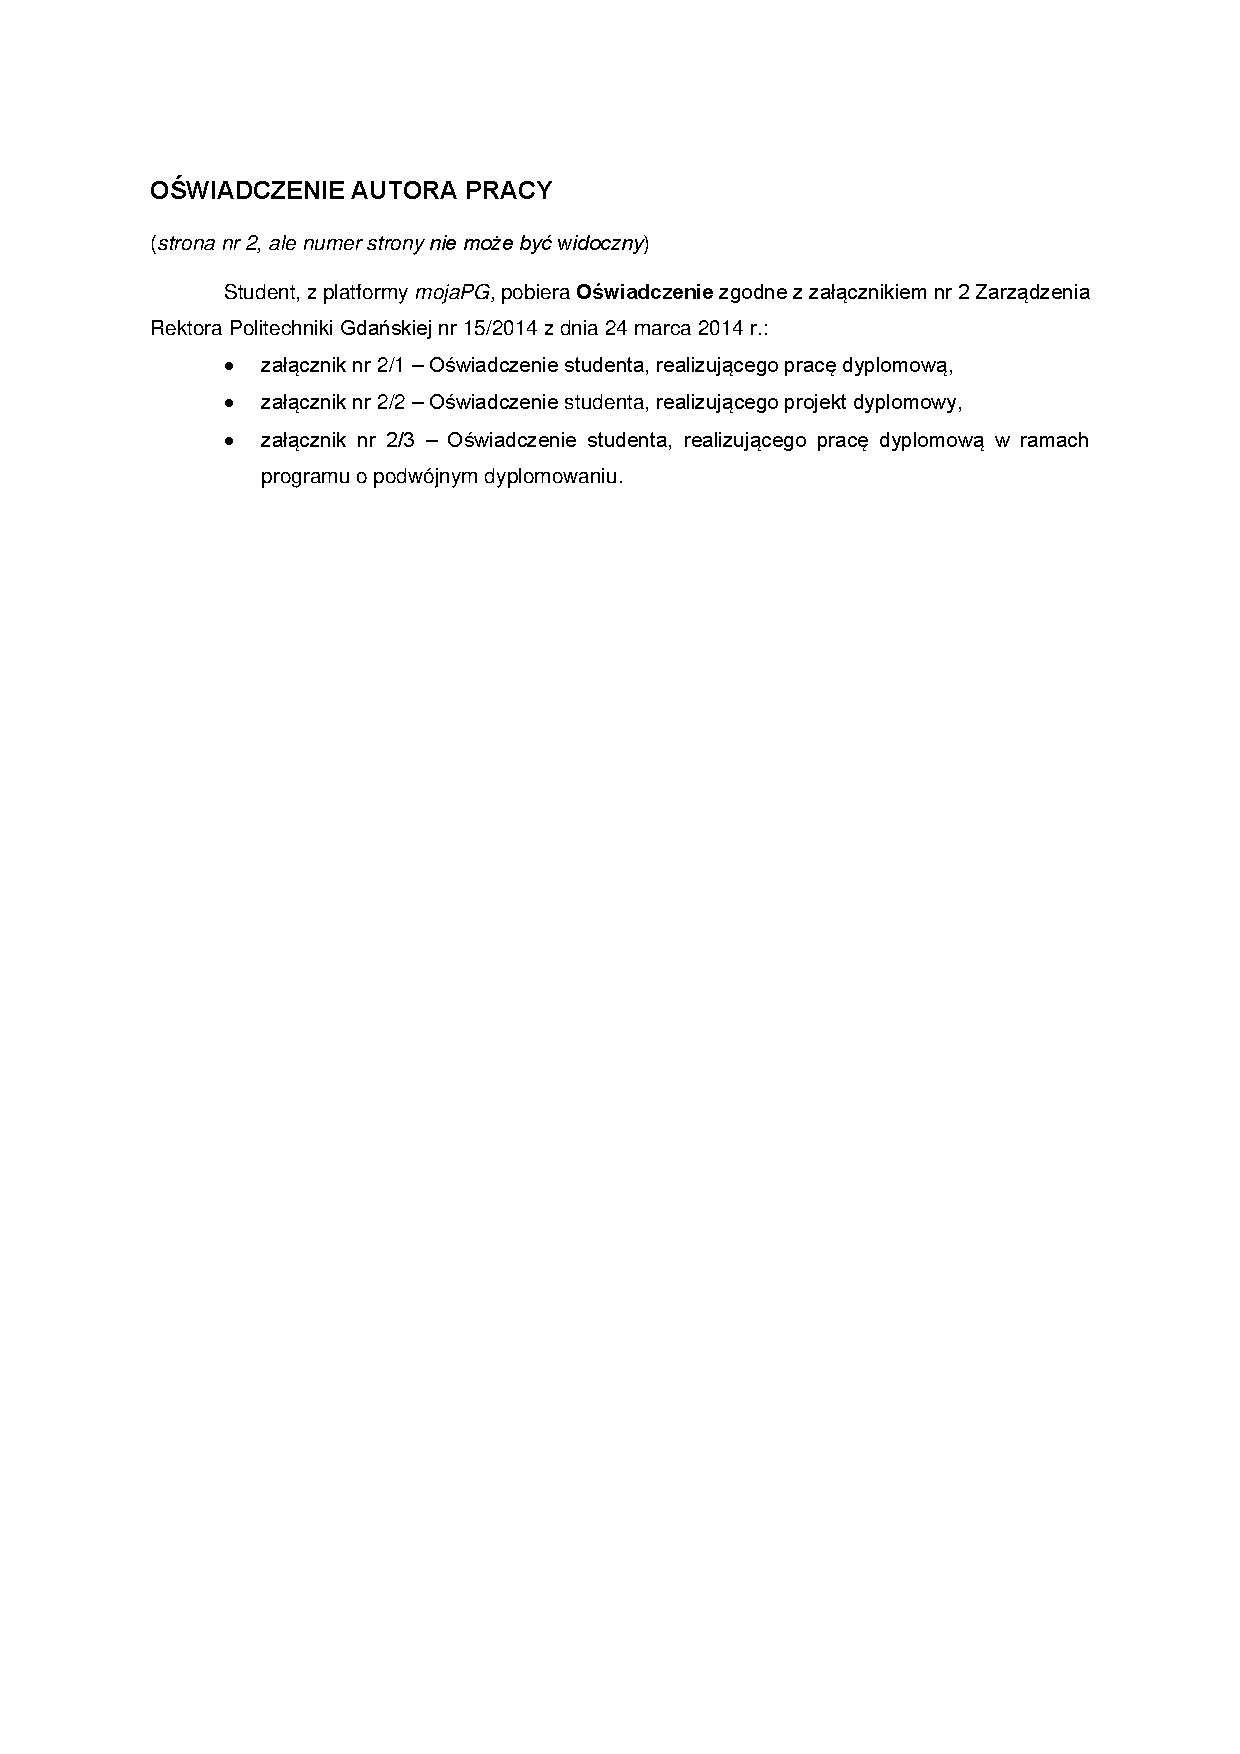
\includepdf{Chapters/Oswiadczenie.pdf}

% streszczenie PL, EN
\chapter*{Streszczenie}
\thispagestyle{plain}

(maksymalnie 1 strona, strona nr 3, numer widoczny)

Streszczenie powinno zawierać określenie problemu naukowego lub praktycznego do rozwiązania, cel i zakres pracy, zastosowane metody badań, wyniki i najważniejsze wnioski.

Jeżeli praca jest realizowana przez co najmniej 2 studentów, to w Streszczeniu należy określić indywidualny udział każdego studenta w realizowanej pracy, podając jakie zagadnienia przez każdego ze studentów zostały opracowane i wykonane. Należy również zamieścić informację jakie rozdziały lub podrozdziały dany student opracował (patrz Spis treści). Należy przyjąć, że punkty podrozdziałów muszą być opracowywane przez studenta odpowiedzialnego za realizację podrozdziału. Przykładowo, jeżeli praca jest realizowana przez studenta A i studenta B, to można przytoczyć zapis: imię i nazwisko studenta A – udział w rozdziałach 1, 7 oraz indywidualnie rozdział 2 oraz podrozdziały 3.1 i 4.2, itd., imię i nazwisko studenta B – udział w rozdziałach 1, 7 oraz indywidualnie rozdział 5 i 6 oraz podrozdziały 3.2 i 4.1, itd.

Celem pracy było wytworzenie aplikacji wspomagającej planowanie i realizację zadań, która wykorzystuje metodologię Geting Things Done autorstwa Davida Allena. Aplikacja ta powinna działać w rozproszonej architekturze w oparciu o łańcuch bloków (ang. Blockchain). 
\\\\
Słowa kluczowe: Blockchain, zdecentralizowany, planowanie
\\\\
Dziedzina nauki i techniki, zgodnie z wymogami OECD: . Nauki inżynieryjne i techniczne, Sprzęt komputerowy i architektura komputerów

\chapter*{Abstract}

The goal of the project was to create a system that supports task planning and execution, as well as enabling text communication between users. The task planning and execution support part was developed based on the Getting Things Done methodology by David Allen.

The main premise of the application was decentralization, so communication was implemented using a distributed architecture based on a Peer-to-Peer network. Data is stored using blockchain technology. Consensus is achieved through the proof of stake algorithm.

These solutions enhance the application's security because they significantly complicate data eavesdropping, impersonation, or manipulation of existing data. They also reduce the risk of data loss as there are multiple storage units. Data is transmitted via the HTTP protocol. It is also encrypted and electronically signed, which further increases security.

The application's interface was written in the QT framework, while the business logic was implemented in Python.
\\\\
Keywords: Blockchain, decentralization, planning, security

% spis treści
\tableofcontents

% wykaz skrótów
\chapter*{Wykaz ważniejszych oznaczeń i skrótów}
\addcontentsline{toc}{chapter}{Wykaz ważniejszych oznaczeń i skrótów}

% otoczenie abbrev zdefiniowane w macra.sty
\begin{abbrev}
\item[Klient] Instancja programu obsługiwana przez danego użytkownika
\item[P2P] Sieć typu peer-to-peer (równy z równym)
\item[IDE] Integrated Development Environment (Zintegrowane Środowisko Programistyczne)
\item[HTTP] Hypertext Transfer Protocol (Protokół Transmisji Hipertekstu)
\item[HTML] HyperText Markup Language (Hipertekstowy Język Znaczników)
\item[CSS] Cascading Style Sheets (Kaskadowe Arkusze Stylów)
\item[UTF-8] 8-bit Unicode Transformation Format (8-bitowy Format Transformacji Unicode)
\item[Backend] Warstwa przechowywania danych i logiki biznesowej
\item[ASCII] American Standard Code for Information Interchange (Amerykański Standardowy Kod Wymiany Informacji)
\item [SHA-256] 256-bit Secure Hash Algorithm (256-bitowy Bezpieczny Algorytm Haszujący)
\item[IEEE] Institute of Electrical and Electronics Engineers (Instytut Inżynierów Elektryków i Elektroników)
\item[IPFS] InterPlanetary File System (Międzyplanetarny System Plików)
\item[RSA] Algorytm Rivesta-Shamira-Adlemana
\item[AES] Advanced Encryption Standard (Zaawansowany Standard Szyfrowania)
\item[DES] Data Encryption Standard (Standard Szyfrowania Danych)
\item[PoS] Proof of Stake (Dowód Stawki)
\item[PoW] Proof of Work (Dowód Pracy)
\item[DPoS] Delegated Proof of Stake (Delegowany Dowód Stawki)
\item[PoC] Proof Of Capacity (Dowód Pojemności)
\item[GTD] Getting Things Done (Załatwianie Spraw)
\item[NIST] National Institute of Standards and Technology (Narodowy Instytut Norm i Technologii)
\item[RC6] Rivest cipher 6 (Szyfr Rivesta 6)
\item[MARS] Multiplication, Addition, Rotation, and Substitution  (Mnożenie, dodawanie, obrót i podstawianie)
\item[TLS] Transport Layer Security (Bezpieczeństwo Warstwy Transportowej)
\item[IPsec] Internet Protocol Security (Bezpieczeństwo Protokołu Internetowego)
\item[WPA] Wi-Fi Protected Access (Dostęp Chroniony Wi-Fi)
\item[ECB] Electronic Code Book (Tryb Elektronicznej Książki Kodowej)
\item[CBC] Cipher Block Chaining (Tryb Wiązania Bloków Zaszyfrowanych)
\item[CFB] Cipher Feedback (Tryb Sprzężenia Zwrotnego Szyfrogramu)
\item[OFB] Output Feedback (Tryb Sprzężenia Zwrotnego Wyjścia)
\end{abbrev}



% rozdziały i podrozdziały numerowane
\chapter{Wstęp i cel pracy}
\label{chap:wstep}
\textit{Autorzy: Maksym Nowak, Piotr Noga}
\par Celem naszej pracy jest wytworzenie aplikacji, która będzie wspomagać użytkowników programu w planowaniu oraz realizacji zadań przy wykorzystaniu metodologii Getting Things Done (GTD), opracowanej przez Davida Allena w jego książce o tym samym tytule \cite{GTD}. GTD to sposób odpowiedniego uporządkowywania planów i zadań tak, aby osoba mogła się skupić na ich realizacji, aniżeli na ciągłym myśleniu o nich \cite{DAllInt}. Jednym z głównych założeń naszego programu jest jego decentralizacja działania, tj. żaden klient nie pełni równocześnie funkcji centralnego serwera, przez który przepływają informacje do innych klientów. Każdy klient łączy się bezpośrednio z pozostałymi, którzy są połączeni ze sobą w sieci typu peer-to-peer (P2P). Z tym sposobem komunikacji klientów związany jest również sposób przechowywania danych, przekazywanych między nimi, gdyż w tym celu zostanie wykorzystana struktura danych zwana łańcuchem bloków (ang. Blockchain).

\section{Uzasadnienie potrzeby realizacji tematu}
Obecnie nie stanowi problemu znalezienie odpowiadającgo użytkownikowi narzędzia do planowania i realizacji zadań w oparciu o metodologię GTD \cite{GTD-apps}. Przykładami takich programów są m.in.:
\begin{itemize}
    \item Nirvana,
    \item Evernote,
    \item ClickUp,
    \item ToodleDo.
\end{itemize}
Programy te jednak mają jedną zasadniczą wadę, które zmotywowały nasz zespół do realizacji tego tematu: żadne z nich nie oferuje możliwości pracy w sposób zdecentralizowany. Mogą one działać jedynie na dwa sposoby:
\begin{itemize}
    \item korzystając z centralnego serwera,
    \item lokalnie.
\end{itemize}
Korzystanie z centralnego serwera oznacza, że użytkownik musi przesyłać dane na serwer firmy zarządzającej danym programem, co może wiązać się z naruszeniem jego prywatności, gdyż wgląd do danych mogą mieć również nieupoważnione osoby. Aplikacje działające lokalnie natomiast mają ograniczenie w postaci możliwości korzystania z nich tylko przez danego użytkownika w odrębie jednego urządzenia, zatem nie ma on możliwości udostępnienia swoich planów czy zadań z innymi upoważnionymi osobami.
\par Bliźniaczo podobna sytuacja ma się z aplikacjami zdecentralizowanymi. Tutaj również można znaleźć pełno rozwiązań spełniających to założenie, lecz żadne z nich nie implementuje w znacznym stopniu GTD. Można zatem stwierdzić, że w momencie redagowania niniejszej pracy dyplomowej, nie istnieje żadne takie rozwiązanie publicznie dostępne, które spełniałoby w pełni nasze wymagania.

\section{Podział prac}
W naszej pracy dyplomowej można wyodrębnić zadania poszczególnych członków w następujący sposób:
\begin{itemize}
    \item Bartosz Kołakowski:
        \begin{itemize}
            \item Lider grupy, odpowiedzialny za koordynowanie pracy i przydzielanie zadań całemu zespołowi. Zrealizował moduł szyfrowania i deszyfrowania wykorzysywany w logice biznesowej naszego programu. Zaimplementował również uzyskiwanie konsensusu PoS. Zmodyfikował w znacznym stopniu działanie mechanizmów związanych z Blockchainem 
        \end{itemize}
    \item Piotr Noga:
        \begin{itemize}
            \item Zrealizował pozostałe komponenty logiki biznesowej programu oraz połączenie jej z interfejsem graficznym.  
        \end{itemize}
    \item Michał Mróz:
        \begin{itemize}
            \item Zrealizował projektowanie i implementację wyglądu aplikacji oraz połączenie interfejsu graficznego z częścią logiki biznesowej aplikacji.  
        \end{itemize}
    \item Maksym Nowak:
        \begin{itemize}
            \item Zrealizował implementację interfejsu graficznego.  
        \end{itemize}
\end{itemize}
\chapter{Stan wiedzy}
\label{chap:stan_wiedzy}
\textit{Autor: Piotr Noga}
\par Zanim podjęliśmy się naszej pracy dyplomowej, przejrzeliśmy artykuły naukowe, literaturę oraz dostępne w Internecie implementacje projektów związanych z naszym tematem pracy. Mogliśmy w ten sposób ugruntować swój stan wiedzy.
\section{Artykuły naukowe}
\label{sec:ArtykulyNaukowe}
Zacznijmy od przeglądu artykułów naukowych. Skupiliśmy swoją uwagę głównie na artykuły naukowe napisane w języku angielskim, lecz staraliśmy się znaleźć również publikacje polskojęzyczne. W poszukiwaniu odpowiednich artykułów naukowych skorzystaliśmy z udostępnianego przez Bibliotekę Politechniki Gdańskiej dostępu do zagranicznych bibliotek cyfrowych. Tymi bibliotekami, z których głównie korzystaliśmy, były:
\begin{itemize}
    \item IEEE Xplore
    \item ACM Digital Library
    \item Springer
    \item Scopus | Elsevier
\end{itemize}
Korzystaliśmy również z ogólnodostępnych bibliotek cyfrowych oraz wydawnictw, oferujących artykuły napisane w języku polskim, takich jak:
\begin{itemize}
    \item Google Scholar
    \item Polska Bibliografia Naukowa
    \item MDPI
\end{itemize}
Swoje poszukiwania rozpoczęliśmy od sprawdzenia, czy istnieją artykuły naukowe odnoszące się w całości do naszego tematu pracy. Mimo próby znalezienia odpowiednich artykułów  poprzez używanie różnych fraz kluczowych w języku polskim, jak również w angielskim, takich jak: "\textbf{system} \ang{system}, \textbf{dispersion} \ang{support}, \textbf{planowanie} \ang{planning}, \textbf{zdecentralizowany} \ang{decentralized}, \textbf{aplikacja} \ang{application}, \textbf{poufność} \ang{confidentiality}, \textbf{niezaprzeczalność} \ang{non-repudiation}, \textbf{rozproszenie} \ang{distributed}, \textbf{konsensus} \ang{consensus}, \textbf{łańcuch bloków} \ang{blockchain}, GTD (skrót od Getting Things Done)", w żadnej z bibliotek nie ma ani jednego artykułu naukowego, który wprost omawiałby aplikację, która implementuje wszystkie założenia naszego systemu. Można znaleźć artykuły odnoszące się jedynie do wybranych zagadnień. Wśród nich można wyróżnić prezentacje implementacji aplikacji zdecentralizowanych. Natrafiliśmy również na jeden z takich artykułów \cite{EvolutionOfBlockchainCon}, który zdecydowanie wpłynął na nasz wybór algorytmu uzgadniania konsensusu łańcuchów bloków, gdyż w szczegółowy sposób omówił każdy z nich, porównał je między sobą, wypisując ich wady i zalety oraz zawierał od razu odnośniki również do innych prac naukowych, w których zostały omówione poszczególne algorytmy.

\section{Literatura}
\label{sec:Literatura}
W przypadku literatury sprawa wygląda podobnie co przy artykułach naukowych. Nie ma takich publikacji, które łączyłyby większość zagadnień związanych z naszą pracą dyplomową, a co najwyżej tylko kilka z nich. Nie mniej jednak można przebierać w wielu książkach związanych z łańcuchem bloków takich jak chociażby "Mastering Blockchain" \cite{MasteringBlockchain}, "Blockchain, Crypto and DeFi" \cite{BCDF}, "Build Your Own Blockchain" \cite{BuildBlockchain} czy też "Bubble Or Revolution?" \cite{BubbleOrRevolution}, które często tłumaczą to zagadnienie w mniej bądź bardziej techniczny sposób, lecz z pewnością w wystarczającym dla nas w zupełności, co z pewnością przyłożyło się na zastosowanie tej struktury danych. Nieodzowną pomocą w naszej pracy okazała się także książka autorstwa Davida Allena pt. "Getting Things Done" \cite{GTD}, która w kompleksowy sposób wyjaśniła nam zasady stojące za tytułową metodologią, którą wdrożyliśmy w naszej aplikacji. Jeśli chodzi o wiedzę kryptograficzną to korzystaliśmy z książek "Kryptografia: w teorii i w praktyce" \cite{KryptografiaWTeoriiPraktyce}, "Kryptografia i ochrona danych" \cite{KryptografiaOchronaDanych} i "Algorytmy kryptograficzne" \cite{AlgorytmyKryptograficzne}. Książki przedstawiające tematykę kryptowalut i zawartych w nich mechanizmów to między innymi "Blockchain. Przewodnik po łańcuchu bloków." \cite{BlockchainPrzewodnikPoLanuchu}, "Blockchain. Fundament nowej gospodarki" \cite{BlockchainFundamentGospodarki} i "Dowód stawki" \cite{DowodStawki}. O aplikacjach zdecentralizowanych i kominukacji równy z równym (peer-to-peer) dowiedzieliśmy się z książek "Projektowanie systemów rozproszonych" \cite{ProjektowanieSystemowRozproszonych} i "Peer-to-Peer. Harnessing the Power of Disruptive Technologies" \cite{PeerToPeer}. Wiedzę o tworzeniu aplikacji internetowych (głownie za pomocą platformy programistycznej Flask) uzyskaliśmy z "Flask. Tworzenie aplikacji internetowych w Pythonie" \cite{FlaskTworzenieAplikacji}, "Mastering Flask" \cite{MasteringFlask} i "Flask By Example" \cite{FlaskExample}. Przy tworzeniu graficznego interfejsu użytkownika (GUI) korzystaliśmy z takich źródeł - "Tkinter GUI Application Development Cookbook" \cite{TkinterCookbook}, "Biblioteki Qt. Zaawansowane programowanie przy użyciu C++" \cite{BibliotekiQt} i "Qt5 Python GUI Programming Cookbook" \cite{QTPython}. %TODO: Również przydatnym zasobem wiedzy były książki zahaczające o tematykę aplikacji zdecentralizowanych.


\section{Projekty użytkowników}
\label{sec:ProjektyUzytkownikow}
Wśród innych entuzjastów technologii, którzy dzielą się z innymi swoimi projektami, znaleźć można różnorakie programy, które w mniejszym lub większym stopniu spełniają założone przez nas cele pracy dyplomowej. Jednymi z najbliższych naszemu programowi są implementacje programów zdecentralizowanych, które posiadają wbudowany moduł planowania zadań, bądź moduł czatu. Przykładami takich programów są "ToDo-DApp" \cite{ToDo_DApp} i "DAPP-todo" \cite{DAPP_todo} w przypadku modułu planera oraz odnośnie modułu czatu "chatDapp" \cite{chatDapp} i "dappchat" \cite{dappchat}. Inną przydatną implementacją był "BlockChat" \cite{blockchat}, w którym była możliwość wysyłania wiadomości przez sieć, a następnie tworzenie z nich bloków opartych na dowodzie pracy jako algorytmie osiągania konsensusu. Inną implemntacją opartą o architekturę rozproszoną i blockchain jest \cite{PythonBlockchain}. To tylko kilka z przykładowych projektów, gdyż nie sposób jest ich zliczyć, lecz wszystkie z nich, jakie przejrzeliśmy, nie łączyły ze sobą obu tych części ze sobą.%TODO

\section{Rozwiązania komercyjne}
\label{sec:RozwiazaniaKomercyjne}
By dopełnić swój stan wiedzy, przejrzeliśmy również jakie są dostępne obecnie na rynku komercyjne rozwiązania, które spełniają jedne z naszych celów. Warto wspomnieć, o platformie zrealizowanej ze środków publicznych (budżet około 5 milionów \cite{IDB})  "lubbezposrednio.pl" \cite{lubBezPosrednio}, która umożliwia głosowanie elektroniczne z wykorzystaniem technologii blockchain. Jednak, tak jak w poprzednich sekcjach nie da się znaleźć żadnego takiego produktu, który umożliwiałby wspomaganie planowania zadań i ich realizacji, który działałby w sposób zdecentralizowany oraz rozproszony. %TODO 

\section{Podsumowanie stanu wiedzy}
\label{sec:PodsumowanieWiedzy}
Podsumowując wszystkie zabrane informacje o obecnym stanie wiedzy, nasuwa się następująca myśl - obecnie nie ma rozwiązania które spełniałoby wszystkie porządane cechy - wspomaganie planowania zadań i ich realizacji, umożliwienie pracy w sposób zdecentralizowany, działanie w architekturze rozproszonej, korzystanie z algorytmu osiągania konsensusu i zapewnienie poufności wiadomości użytkowników. Nasza praca dyplomowa ma na celu między innymi zmianę tego stanu rzeczy i wypuszczenie na świat pierwszego produktu w takim stylu.
\chapter{Interfejs graficzny użytkownika}
\label{chap:InterfejsGraficznyUżytkownika}
Aplikacja posiada rozbudowany graficzny interfejs użytkownika, który w sposób responsywny dostosowuje się do urządzeń desktopowych oraz mobilnych. Interfejs dostępny jest w dwóch trybach wizualnych: jasnym i ciemnym, oferując różnorodne efekty kolorystyczne oraz animacje. Dodatkowo aplikacja renderuje dynamicznie pojedynczy obiekt trójwymiarowy wraz z jego animacją, co wzbogaca wizualny aspekt interfejsu.

%---
\section{Projektowanie interfejsu graficznego}
\label{sec:ProjektowanieInterfejsuGraficznego}

\emph{Projektowanie interfejsu graficznego \ang{UI Design}}, to proces tworzenia wizualnego środowiska użytkownika przed jego implementacją programistyczną. W ramach naszego projektu inżynierskiego wykorzystałem profesjonalne narzędzie Figma \cite{Figma} do zaprojektowania interfejsu graficznego użytkownika, co pozwoliło usprawnić i ujednolicić dalsze prace związane z implementacją tego interfejsu w kodzie. Projekt graficzny stworzony w Figmie pełnił funkcję przewodnika, przy programowaniu interfejsu.

%---

\subsection{System Projektowania}
\label{sec:SystemProjektowania}

\emph{System projektowania \ang{Design system}}, to zestaw standaryzowanych danych i zasobów projektowych, które wspólnie definiują wygląd interfejsu graficznego i usprawniają proces projektowania. Celem Design systemu jest zapewnienie spójności wizualnej oraz ułatwienie współpracy między członkami zespołu. 
W ramach projektowania interfejsu graficznego, zacząłem od stworzenia prostego systemu projektowania, który ujednolicił paletę barw, definiując zestawy kolorów o różnych odcieniach jasności, rozmiary czcionek oraz odstępy między elementami. Te wartości stałe były konsekwentnie wykorzystywane zarówno w procesie projektowania, jak i w implementacji interfejsu graficznego, zapewniając spójność wizualną i funkcjonalną. 

%---

\subsection{Proces projektowania}
\label{sec:ProcesProjektowania}
Po zdefiniowaniu Systemu Projektowania rozpocząłem projektowanie stron aplikacji w dwóch rozdzielczościach: 1440x1024 dla urządzeń desktopowych oraz 375x667 dla urządzeń mobilnych. Dla każdej z tych rozdzielczości przygotowałem dwie wersje stron, różniące się układem elementów. Wszystkie projekty początkowo powstawały w kolorystyce \ang{Dark Mode}, a następnie były tworzone ponownie w jasnej wersji \ang{Light Mode}.

%---

\section{Implementacja Interfejsu Graficznego}
\label{sec:ImplementacjaInterfejsuGraficznego}
Język Python posiada wiele bibliotek do tworzenia interfejsów graficznych, nasz zespół zdecydował się na użycie frameworka QT w wersji 6 (Pyside6). Dzięki temu, że framework stanowi pakiet w języku Python nasz zespół mógł używać różnych IDE \ang{Integrated Development Environment}.
Framework ten posiada wiele narzędzi i komponentów umożliwiających tworzenie nie tylko interfejsów graficznych, od własnych struktur danych po moduły do pracy z bazami danych, jednakże w naszym projekcie głównie korzystaliśmy z języka Qt do Modelowania (QML) \ang{Qt Modeling Language} - deklaratywnego języka do tworzenia interfejsów w Frameworku QT. QML oraz QT jest wieloplatformowy, działa na urządzeniach desktopowych (Windows, Linux, MacOS) oraz urządzeniach mobilnych i wiele innych.
Dzięki QML możliwe było logiczne rozdzielenie backendu i frontendu, co pozwoliło na zapisanie definicji interfejsu graficznego w odrębnych plikach z rozszerzeniem .qml, ułatwiając tym samym zarządzanie kodem i jego strukturą.

\subsection{Uzasadnienie wyboru Frameworka QT}
\label{sec:UzasadnienieWyboruFrameworkaQT}
Przy wyborze technologii do tworzenia interfejsów graficznych w Pythonie mieliśmy do wyboru wiele innych bibliotek, na przykład Tkinter. 
Jednakże w porównaniu do Tkintera, interfejsy w tej bibliotece są przestarzałe wizualnie i mniej elastyczne. Biblioteka ta oferuje małe wsparcie dla chociażby efektów wizualnych, animacji czy responsywnego designu.

Framework QT oraz zawarty w nim QML mają wiele zalet, które nas przekonały do skorzystania z tej technologii:
\begin{enumerate}
    \item Qt jest wieloplatformowy, można tworzyć aplikacje na Windowsa, Linuxa, MacOSa i urządzenia mobilne
    \item Łatwo łączyć logikę backendu z frontendem
    \item QML umożliwia dodawanie animacji, renderowanie obiektów trójwymiarowych i tworzenie responsywnego interfejsu
    \item QT posiada ogromną dokumentację i ma szeroką społeczność użytkowników
    \item Oddzielenie frontendu (QML) od backendu (Python) sprzyja lepszej organizacji kodu
\end{enumerate}

\subsection{Podstawy QT Modeling Language} 
\label{sec:PodstawyQtModelingLanguage}
\emph{Qt Modeling Language} to język deklaratywny podobny do CSS i HTML, wchodzący w skład modułu QtQuick frameworka Qt. Aby zacząć używać QML'a, należy stworzyć plik .qml w którym możemy zawrzeć:

\begin{lstlisting}[language=QML, caption={Przykładowy kod QML}]
import QtQuick 2.0

Rectangle {
    id: kwadrat
    width: 100
    height: 100
    color: "red"
}
\end{lstlisting}
który tworzy kwadrat 100x100 w kolorze czerwonym, struktura kodu w QML jest hierarchiczna oznacza to, że wewnątrz kodu Rectangle moglibyśmy dodać kolejny obiekt, który byłby tworzony względem rodzica - Rectangle.

Dodatkowo QML umożliwia pisanie w języku Javascript w odpowiednich polach,
na przykład do kodu w kwadracie można dodać:

\begin{lstlisting}[language=QML, caption={Przykładowy Javascript}]
Component.onCompleted: {
    console.log(kwadrat.width);
}
\end{lstlisting}
który wypisze w konsoli szerokość kwadratu.


\subsection{Zaimplementowane istotne mechanizmy}
\label{sec:ZaimplementowaneIstotneMechanizmy}

\subsubsection{Struktura Interfejsu}
\label{sec:Struktura Interfejsu}
W naszym projekcie każdy osobny plik .qml stanowi osobną stronę interfejsu lub
definicję niestandardowego komponentu. Niestandardowe komponenty są zawarte
w osobnych folderach: \begin{lstlisting}
"app_style", "gui_components", "small_gui_components"
\end{lstlisting}

Omówię najpierw aspekt niestandardowych komponentów. W QMLu można tworzyć własne klasy komponentów.

\begin{lstlisting}[language=QML, caption={Przykładowa klasa w MyRectangle.qml}]
MyRectangle {
    id: rectangle
    color: "blue"
    width: 100
    height: 100
}
\end{lstlisting}
Zaimportowanie tego w innym pliku (Page1.qml) umożliwi stworzenie
wielu instancji klasy MyRectangle:

\begin{lstlisting}[language=QML, caption={Przykładowe użycie klasy MyRectangle}]
MyRectangle {} //niebieski kwadrat 100x100
MyRectangle {color: "red"} //czerwony kwadrat 100x100
\end{lstlisting}
Pozwala to na uniknięcie redundancji w kodzie, gdy trzeba tworzyć
wiele obiektów, różniących się, tylko niektórymi atrybutami.

W naszym projekcie jest to wykorzystywane przy tworzeniu list, na przykład
użytkowników albo własnych przycisków, których w interfejsie jest pełno i dzięki definiowaniu ich w jednej klasie, wyglądają podobnie i upraszczają kod.

Reszta plików \texttt{.qml} stanowi osobne strony interfejsu. 
Tworząc komponent StackView oraz używając:
\begin{lstlisting}[language=QML, caption={Ładowanie nowej strony}]
stackView.push("nazwa_pliku.qml");
\end{lstlisting}
można w bardzo prosty sposób załadować nową stronę.
Taki podział (strona - plik) sprawia, że struktura interfejsu jest bardziej
uporządkowana oraz logiczna i upraszcza pracę z kodem.

\subsubsection{Implementacja Systemu Projektowania}
\label{sec:ImplementacjaSystemuProjektowania}
System Projektowania z części Projektowania Interfejsu Graficznego zakłada użycie stałej palety kolorów, odstępów oraz wielkości czcionek.

Nasz projekt implementuje to w folderze \texttt{app\_style} w trzech plikach QML:

\begin{enumerate}
    \item ColorPalette.qml - Definiujący zestaw stałych kolorów
    \item FontStyle.qml - Definiujący czcionkę oraz różne rozmiary
    \item SpacingObjects.qml - Definiujący wartości odstępów między elementami w interfejsie
\end{enumerate}

Każdy z nich zawiera analogiczną logikę, więc omówię na przykładzie klasy \texttt{ColorPalette}:

W kodzie QML definiujemy stałe zmienne przy użyciu \texttt{property}

\begin{lstlisting}[language=QML, caption={ColorPalette.qml}]
import QtQuick 2.15

QtObject {
    readonly property color primary50: "#EBFFE5"
    readonly property color primary100: "#D7FFCC"
    readonly property color primary200: "#AFFF99"
    readonly property color primary300: "#87FF66"
    readonly property color primary400: "#5FFF33"
    readonly property color primary500: "#37FF00"
    readonly property color primary600: "#2CCC00"
    readonly property color primary700: "#219900"
    readonly property color primary800: "#166600"
    readonly property color primary900: "#0B3300"

    readonly property color secondary50: "#FEE5FF"
    readonly property color secondary100: "#FDCCFF"
    ...
    ...
\end{lstlisting}

Następnie w bardzo prosty sposób możemy używać tych stałych wartości w każdym miejscu w kodzie:
\begin{lstlisting}[language=QML, caption={Przykładowe użycie palety kolorów}]
import "../app_style"

//User (Peer) List Class Blueprint
Rectangle {
ColorPalette { id: colorPalette }
FontStyle { id: fontStyle }
SpacingObjects { id: spacingObjects }

    property string list_color: settings.light_mode ? colorPalette.background50 : colorPalette.background800
    ...
    ...
\end{lstlisting}  

\subsubsection{Komunikacja z Backendem}
\label{sec:KomunikacjaZBackendem}
Komunikacja z backendem w Frameworku QT odbywa się za pomocą sygnałów i slotów. Ten sam mechanizm istnieje również, gdy używamy QT wraz z językiem C++, jednakże syntax jest inny. 

Sygnał to obiekt, który jak nazwa wskazuje ma za zadanie wysłanie sygnału,
dokonuje się tego przy pomocy metody .emit().

Slot to specjalna funkcja, którą należy połączyć z wybranym, uprzednio stworzonym sygnałem.

Po wysłaniu sygnału zostaje wywołany ten podłączony Slot. Dodatkowo można przesyłać w metodzie .emit() argumenty do Slota.

Jeżeli chcemy osiągnać komunikację między backendem (plikami .py) oraz frontendem (.qml) to logicznie:

\begin{enumerate}
    \item Definiujemy sygnał w klasie w Pythonie, który potem należy podłączyć do zdefiniowanej w QML-u za pomocą JavaScript funkcji (slota) i następnie wywołać \texttt{.emit()} z poziomu Pythona dla tego sygnału. To umożliwi wywołanie funkcji zawartej w QML za pomocą kodu w Pythonie.
    \item Możemy też pójść w drugą stronę – jeśli chcemy wywołać coś z backendu przy użyciu kodu QML, wtedy należy stworzyć slot w klasie w Pythonie, gdzie kod QML staje się sygnałem.
\end{enumerate}

Istotnym aspektem jest to, że samo przekazanie wartości do frontendu jest operacją prostą, można tego dokonać jednorazowo przy inicjalnym ładowaniu interfejsu, o czym za chwilę, jednakże mechanizm sygnałów i slotów umożliwia dynamiczne przekazywanie informacji między frontendem i backendem.

Na przykład jeśli dodamy kogoś do znajomych, to w backendzie w funkcji która odpowiada za dodanie użytkownika do znajomych możemy wywołać .emit() i dynamicznie obsłużyć tą zmianę we Frontendzie.

Teraz pokazując kod z naszego projektu omówię na przykładzie jak wykorzystaliśmy ten mechanizm:

Przykładowo jeśli dynamicznie obsłużyć zmianę znajomych w naszym programie, to atrybut self.peers w klasie User() w Backendzie zawiera tablicę innych obiektów typu User, które chcemy przekazać do Frontendu i wypisać na ekranie.

Tworzymy sygnał w klasie User:
\begin{lstlisting}[language=Python, caption={Sygnał User}]
class User(QObject):
    peersChanged = Signal()
\end{lstlisting}    

Definiujemy tablicę peers jako Property:
\begin{lstlisting}[language=Python, caption={Peers Property}]
@Property("QVariantList", notify=peersChanged)
    def peers(self):
        return self._peers
\end{lstlisting}

W main.py przed inicjalnym załadowaniem interfejsu możemy przekazać
uprzednio stworzony pojedyńczy obiekt User, gdzie u nas jest to obecny użytkownik programu. Teraz w QML możemy używać metod i atrybutów tej klasy dla tego obiektu.

\begin{lstlisting}[language=Python, caption={Przekazanie inicjalnego obiektu}]
engine.rootContext().setContextProperty("user", user)
\end{lstlisting}

Teraz w klasie FriendList, po załadowaniu komponentu należy podłączyć sygnał peersChanged z funkcją javascript, która przetwarza dane znajomych z obiektu user.

\begin{lstlisting}[language=Python, caption={Podłączenie sygnału do slota w QML}]
Component.onCompleted: {
        user.peersChanged.connect(updateUserModel);
}
\end{lstlisting}
Teraz każdy peersChanged.emit() w pythonie spowoduje wywołanie funkcji updateUserModel, która u nas w projekcie, wygląda tak:

\begin{lstlisting}[language=Python, caption={Slot w QML obsługujący wyświetlanie zmienionej listy znajomych}]
function updateUserModel() {
    userModel.clear();

    // Iterate over peers array passed from Python
    for (let i = 0; i < user.peers.length; i++) {
        var activeColor = user.peers[i].active > 0 ? colorPalette.primary500 : colorPalette.destructive400

        var isInGroup = false;
        var isSelected = false;

        var host = user.peers[i].host;
        var port = user.peers[i].port;

        for (let j = 0; j < user.group.length; j++) {
            if (host === user.group[j].host && port === user.group[j].port) {
                isInGroup = true;
                break;
            }
        }

        userModel.append({
            nickname: user.peers[i].nickname,
            host: host,
            port: port,
            active: user.peers[i].active,
            isInGroup: isInGroup,
            isSelected: isSelected,
            activeColor: activeColor
        });
    }
}
\end{lstlisting}
Dla uproszczenia można założyć, że userModel to po prostu lista znajomych.
W ten sposób możemy dynamicznie aktualizować wyświetlane dane w Frontendzie za każdym razem, gdy lista znajomych (self.peers) ulegnie zmianie.

Na przykład funkcja odpowiadająca za usunięcie znajomego, która jest Slotem - wywoływana jest z poziomu Frontendu po kliknięciu przycisku, a Backend informuje Frontend o usunięciu znajomego za pomocą .emit(), a ten następnie przetwarza tą zmianę i wyświetla na ekranie:
\begin{lstlisting}[language=Python, caption={Przykładowe użycie sygnału dla listy znajomych}]
@Slot(str, int)
def removeFromPeers(self, host, port):
    for peer in self.peers:
        if peer.host == host and peer.port == port:
            self.peers.remove(peer)
            self.peersChanged.emit()
            break
\end{lstlisting}

\subsubsection{Renderowanie Obiektu Trójwymiarowego}
\label{sec:RenderowanieObiektuTrójwymiarowego}
Nasza aplikacja renderuje jeden obiekt trójwymiarowy, istotne jest to, że korzystamy z dynamicznego renderera obiektów 3D zamiast na przykład prostego .gifa.
QT umożliwia renderowanie obiektów 3D w QMLu, przy użyciu modułu Qt3D, który w naszym projekcie umożliwia narysowanie trójwymiarowego kształtu i jego animacje (obrót do okoła osi Y)

Przedstawię kod odpowiedzialny za to i następnie go omówię:
\begin{lstlisting}[language=QML, caption={Renderowanie trójwymiarowego bitcoina}]
View3D {
    id: view3D
    Layout.alignment: Qt.AlignHCenter
    anchors.fill: parent
    environment: sceneEnvironment

    SceneEnvironment {
        id: sceneEnvironment
        antialiasingQuality: SceneEnvironment.High
        antialiasingMode: SceneEnvironment.MSAA
    }

    Node {
        id: scene
        DirectionalLight {
            id: directionalLight
        }

        PerspectiveCamera {
            id: sceneCamera
            x: 0
            y: 0
            z: 500
        }

        Bitcoin {
            id: bitcoin

            x: -scale.x * 0.5
            y: -scale.y * 2
            z: -scale.z * 1

            property var scaleFactor: Math.sqrt(Math.min(root.width, root.height)) * 5

            scale: Qt.vector3d(scaleFactor, scaleFactor, scaleFactor)
        }
    }

    NumberAnimation {
        target: bitcoin
        property: "eulerRotation.y"
        loops: Animation.Infinite
        running: true
        from: 360
        to: 0
        duration: 10000
    }
}
\end{lstlisting}

TODO
...
...

% responsywność interfejsu i skalowanie komponentów
\subsubsection{Responsywność interfejsu}
\label{sec:ResponsywnośćInterfejsu}
TODO

\subsection{Pomoce naukowe związane z QT i QML}
\label{sec:PomoceNaukoweQML}
Przy pracy z Frameworkiem QT i QML korzystaliśmy z ogromnej oficjalnej dokumentacji: 
Dokumentacja QT \cite{DokumentacjaQT}
Dokumentacja QML \cite{DokumentacjaQML}
Dokumentacja QT for Python \cite{DokumentacjaQtForPython}.

Dodatkowo niektórzy członkowie zespołu korzystali z IDE przeznaczonego do pracy w QT: Qt Creator, który ma wbudowaną tą dokumentację i pod ręką na przykład można zaznaczyć obiekt w kodzie i kliknąć "f2", co sprawi, że otworzy się osobne okno w programie z dokumentacją tego obiektu. Z tego również czasem korzystaliśmy.

Dodatkowo korzystaliśmy z poradnika na youtubie:
Poradnik \cite{PoradnikQMLYoutube}

\subsection{Strategie rozwiązywania problemów w QML}
\label{sec:StrategieRozwiązywaniaProblemówWQML}
Podczas pracy w QML napotykaliśmy wiele różnych ciekawych problemów, które z czasem nauczyliśmy się rozwiązywać co raz to bardziej efektywnie.
TODO ...

\chapter{Super rozdział}
\label{chap:super}

Mam tu jeszcze raz tabelę \ang{table}, tym razem to tabela \ref{tab:interakcja}. Poprzednią tabelą była tabela \ref{tab:font_size} - \zobrozdz{chap:wstep}

\begin{table}[!ht]

\caption{Możliwości obliczeniowe współczesnych systemów}
\label{tab:interakcja}
\small
\begin{tabular}{|p{0.47\textwidth}|p{0.47\textwidth}|}
\hline

%-
\begin{center}
\textbf{Wnioski z~hipotezy Turinga}
\end{center}
 & 
\begin{center}
\textbf{Wnioski zaproponowane przez~Wegnera i~Goldin}
\end{center}

\\\hline 

%-
  Wszystkie problemy \emph{obliczalne} można rozwiązać za~pomocą funkcji. &  Wszystkie problemy \emph{algorytmiczne} można rozwiązać za~pomocą funkcji. \\\hline
%-
	Wszystkie problemy \emph{obliczalne} można opisać algorytmem. &  Wszystkie problemy \emph{oparte na~funkcjach} można opisać algorytmem.\\\hline
%-
	Algorytmy są tym, co~mogą wykonywać \emph{dowolne komputery}. & Algorytmy są tym, co~mogły wykonywać \emph{wczesne} komputery. \\\hline
%-
	Maszyna Turinga jest ogólnym modelem \emph{dowolnych} komputerów.  &  Maszyna Turinga jest ogólnym modelem \emph{wczesnych} komputerów.\\\hline
%-
	Maszyna Turinga potrafi zasymulować \emph{dowolny} komputer.  &  Maszyna Turinga potrafi zasymulować \emph{dowolne urządzenie} realizujące algorytmiczne obliczenia.\\\hline
%-
	
	\begin{center}
	\Large{\sffamily{:(}}
	\end{center}
			 &  Maszyna Turinga nie~potrafi rozwiązać każdego problemu obliczeniowego ani wykonać wszystkich operacji, które realizują \emph{współczesne systemy}.\\\hline


\end{tabular}
\end{table}


I może jeszcze logo:

\begin{figure}[!ht]
	\centering
		
\includegraphics[width=0.3\textwidth]{Images/logo_pg.jpg}
	\caption{Oto logo PG}
	\label{fig:PD}
\end{figure}



\chapter{Podsumowanie}
Udało się nam zrealizować wszystkie stawiane systemowi wymagania:
\begin{itemize}
    \item System działa w architekturze rozproszonej, każdy z użytkowników jest równy innym, system został zaimplementowany bez użycia głównego serwera, co pozwoliło uniknąć centralizacji
    \item W systemie można wysyłać wiadomości do innych użytkowników
    \item W systemie można tworzyć grupy z dowolnymi użytkownikami i treść wiadomości dla osób z poza grupy nie jest dostępna
    \item System oparty jest o mechanizmy działające w kryptowalutach mające na celu zapewnienie w nim uczciwości i bezpieczestwa
    \item System posiada graficzny interfejs użytkownika, pozwalający na łatwiejsze korzystanie z niego
    \item System posiada szyfrowanie danych w celu zapewnienia poufności i tego, aby nikt z poza sieci nie mógł odczytać treści wiadmości
    \item W systemie zapewniona jest niezaprzeczalność wiadomości poprzez ich podpisywanie podpisem cyfrowym przez weryfiktora
    \item W systemie zaimplementowane są mechanizmy zapwenianiania uczciwości poprzez implementację algorytmów osiągania konsensusu
    \item W systemie można planować zadania do wykonania
\end{itemize}
\vspace{0.3\baselineskip}
Podsumowując stworzyliśmy działający system z w pełni działającym graficznym interfejsem użytkownika, który pozwala na komunikację między użytkownikami i jak i tworzenie dowolnie dużych grup użytkowników, dla których odbywa się komunikacja grupowa. W systemie zapewniona jest poufność poprzez zastosowanie szyfrowania wiadmości, niezaprzeczalność przez podpisywanie cyfrowe bloków wiadomości i mechanizmy zapewniania uczciwości systemu przez algorytmu osiągania konsensusu.

% bibliografia
% ieeetr - etykiety numerowane w kolejności wystąpienia w tekście
\bibliographystyle{ieeetr}
\bibliography{Chapters/Bibliography}

% wykazy 
\listoffigures
\listoftables

% dodatki
\appendix
% słaba funkcja
% \titlecontents{chapter}[0cm]{}{\normalsize\bfseries{\appendixname\space}\contentslabel{-1pt}\hspace*{0.6cm}}{}{\titlerule*[4.5pt]{.}\hspace*{5pt}\contentspage}

\chapter*{Dodatek A: Uzupełnienie wymogów}
\addcontentsline{toc}{chapter}{Dodatek A}
% Póki co jest problem ze słowem dodatek w spisie treści. Funkcja wklejona na początku działa słabo. Powyższe linijki obchodzą ten problem bardzo dobrze, ale dodatki trzeba sobie numerować "ręcznie"

No i mamy jeszcze dodatek - jeśli trzeba

Dodatki należy oznaczać kolejnymi dużymi literami alfabetu. W dodatkach należy umieszczać elementy uzupełniające, które powinny zostać dołączone do pracy, np. w celu prezentacji wykonanych obliczeń, schematy ideowe.  
\end{document}
